\documentclass[journal,10pt,twocolumn]{article}
\usepackage[margin=0.5in]{geometry}
\usepackage[cmex10]{amsmath}
\usepackage{array}
\usepackage{booktabs}
% The preceding line is only needed to identify funding in the first footnote. If that is unneeded, please comment it out.
\usepackage{cite}
\usepackage{amsmath,amssymb,amsfonts}
\usepackage{graphicx}
\usepackage{textcomp}
\usepackage{xcolor}
\usepackage{graphicx}
\graphicspath{{./fig}}{}
\def\BibTeX{{\rm B\kern-.05em{\sc i\kern-.025em b}\kern-.08em
    T\kern-.1667em\lower.7ex\hbox{E}\kern-.125emX}}
\usepackage{tikz}
\usetikzlibrary{shapes.geometric}
\usetikzlibrary{shapes.geometric,angles,quotes}
\begin{document}
\newtheorem{theorem}{Theorem}[section]
\newtheorem{problem}{Problem}
\newtheorem{proposition}{Proposition}[section]
\newtheorem{lemma}{Lemma}[section]
\newtheorem{corollary}[theorem]{Corollary}
\newtheorem{example}{Example}[section]
\newtheorem{definition}[problem]{Definition}
%\newtheorem{thm}{Theorem}[section] 
%\newtheorem{defn}[thm]{Definition}
%\newtheorem{algorithm}{Algorithm}[section]
%\newtheorem{cor}{Corollary}
\newcommand{\BEQA}{\begin{eqnarray}}
\newcommand{\EEQA}{\end{eqnarray}}
\newcommand{\define}{\stackrel{\triangle}{=}}
\newcommand*\circled[1]{\tikz[baseline=(char.base)]{
    \node[shape=circle,draw,inner sep=2pt] (char) {#1};}}
\bibliographystyle{article}
%\bibliographystyle{ieeetr}
\providecommand{\mbf}{\mathbf}
\providecommand{\pr}[1]{\ensuremath{\Pr\left(#1\right)}}
\providecommand{\re}[1]{\ensuremath{\text{Re}\left(#1\right)}}
\providecommand{\im}[1]{\ensuremath{\text{Im}\left(#1\right)}}
\providecommand{\qfunc}[1]{\ensuremath{Q\left(#1\right)}}
\providecommand{\sbrak}[1]{\ensuremath{{}\left[#1\right]}}
\providecommand{\lsbrak}[1]{\ensuremath{{}\left[#1\right.}}
\providecommand{\rsbrak}[1]{\ensuremath{{}\left.#1\right]}}
\providecommand{\brak}[1]{\ensuremath{\left(#1\right)}}
\providecommand{\lbrak}[1]{\ensuremath{\left(#1\right.}}
\providecommand{\rbrak}[1]{\ensuremath{\left.#1\right)}}
\providecommand{\cbrak}[1]{\ensuremath{\left\{#1\right\}}}
\providecommand{\lcbrak}[1]{\ensuremath{\left\{#1\right.}}
\providecommand{\rcbrak}[1]{\ensuremath{\left.#1\right\}}}
\newcommand{\sgn}{\mathop{\mathrm{sgn}}}
%\providecommand{\hilbert}{\overset{\mathcal{H}}{ \rightleftharpoons}}
\providecommand{\system}{\overset{\mathcal{H}}{ \longleftrightarrow}}
	%\newcommand{\solution}[2]{\textbf{Solution:}{#1}}
\newcommand{\solution}{\noindent \textbf{Solution: }}
\newcommand{\cosec}{\,\text{cosec}\,}
\providecommand{\dec}[2]{\ensuremath{\overset{#1}{\underset{#2}{\gtrless}}}}
\newcommand{\myvec}[1]{\ensuremath{\begin{pmatrix}#1\end{pmatrix}}}
\newcommand{\mydet}[1]{\ensuremath{\begin{vmatrix}#1\end{vmatrix}}}
	\newcommand*{\permcomb}[4][0mu]{{{}^{#3}\mkern#1#2_{#4}}}
\newcommand*{\perm}[1][-3mu]{\permcomb[#1]{P}}
\newcommand*{\comb}[1][-1mu]{\permcomb[#1]{C}}
%\numberwithin{equation}{section}
\numberwithin{equation}{subsection}
%\numberwithin{problem}{section}
%\numberwithin{definition}{section}
\let\vec\mathbf
\title{
{Deriving the equation of Ellipse with eccentricty, directrices\\
and origin as its center\\
Using Matrices}\\
\thanks{Meer Tabres Ali as an intern with FWC IIT Hyderabad. *The author is with the Department of Electrical Engineering, Indian Institute of Technology, Hyderabad 502285 India e-mail: gadepall@iith.ac.in. All content in this manual is released under GNU GPL. Free and open source.}
}
\author{Meer Tabres Ali and G V V Sharma}
\maketitle
\tableofcontents
\section{Problem statement}
The eccentricity of an ellipse, with its center at the origin, is $\frac{1}{2}$. If one of the directrices is $\vec{x}=4$, then find the equation of Ellipse.
\section{Considerations}
\vspace{0.2cm}
As per the statement, for the given Ellipse, the input parameters are described in the following table. \\
\vspace{0.2cm}

\setlength\extrarowheight{2pt}
\begin{tabular}{|c|c|c|}
	\hline
	\textbf{Symbol}&\textbf{Value}&\textbf{Description}\\
	\hline
	$\vec{O}$ & \myvec{0\\0}
	&Origin\\
	\hline
	e & 0.5 & Eccentricity\\
	\hline
	$\vec{x}$ & $\vec{x}=4$
	&Directrix
	\\
\hline
\end{tabular}

\section{Plotting the Ellipse with the given parameters}
\vspace{0.25cm}
The plot of the Ellipse, with eccentricity $\vec{e}$ = 0.5 and directrix ($\vec{x}=4$) is shown in figure below.
\begin{figure}[h]
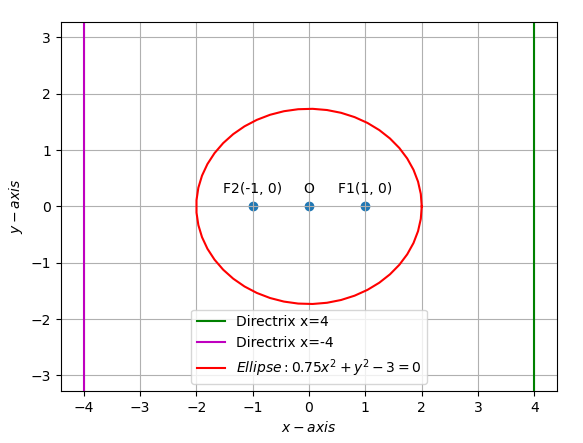
\includegraphics[width=1\columnwidth]{ellipse.png}
\caption{Ellipse with eccentricty e=0.5 and directrix x=4)}
\label{fig:Ellipse}
\end{figure}
\section{Solution}
\vspace{0.25cm}
As per the statement, for the given Ellipse, the input parameters are,\\
\begin{flushleft}
Eccentricity of the Ellipse is,\\
\end{flushleft}
\center
e = 0.5 \\
\endcenter
\begin{flushleft}
And the Directrix of the Ellipse is,\\
\end{flushleft}
\begin{equation}
\vec{x}=4 \label{eq:directrix}
\end{equation}
\begin{flushleft}
On comparing above equation $\eqref{eq:directrix}$ with, $\vec{n}^T\vec{x}=\vec{c}$\\
we get,\\
\end{flushleft}
$\vec{n}=\myvec{1\\0}$ and $\vec{c}=4$\\
\begin{flushleft}
Therefore, the directrix of the Ellipse, $\vec{n}^T\vec{x}=\vec{c}$ can be written as,\\
\vspace{0.2cm}
(where $\vec{n}$ is normal vector of directix line)
\end{flushleft}
\begin{equation}
\implies \myvec{1&0} \vec{x}=4
\end{equation}
\begin{flushleft}

\subsection{Finding the Matrix $\vec{V}$}
\end{flushleft}
\vspace{0.25cm}
\begin{flushleft}
The Matrix $\vec{V}$ can be expressed as,\\
\end{flushleft}
\begin{equation}
\vec{V} =||\vec{n}||^2\vec{I}-e^2\vec{n}\vec{n}^T   
\end{equation}
\begin{flushleft}
On submitting $\vec{n}=\myvec{1\\0}$ and e=$\frac{1}{2}$ in above equation, we get,\\
\end{flushleft}
\endcenter
\begin{center}
$\vec{V} =(1^2)\myvec{1&0\\0&1}-\brak{\frac{1}{2}}^2 \myvec{1\\0} \myvec{1&0}$\\  
\end{center}
\begin{center}
$\implies \vec{V} =\myvec{1&0\\0&1}- \myvec{\frac{1}{4}&0\\0&0}$\\ 
\end{center}
\begin{equation}
   \implies \vec{V}=\myvec{\frac{3}{4} & 0 \\ 0 & 1}
\end{equation}
\begin{flushleft}
\subsection{Finding the Matrix $\vec{u}$}
\end{flushleft}
\vspace{0.2cm}
\begin{flushleft}
As per the statement, Center of the Ellipse is origin,
\end{flushleft}
\begin{equation}
   \implies \vec{O} = \myvec{0\\0}
\end{equation}
\begin{flushleft}
And the center of conics is,\\
\end{flushleft}
\begin{equation}
    \vec{O} = -\vec{V}^{-1} \vec{u}
\end{equation}
\center
$\implies \vec{u} = -\vec{V} \vec{O}$\\
\center
$\implies \vec{u} = -\myvec{\frac{3}{4}& 0\\0&1} \myvec{0\\0}$
\vspace{0.2cm}
\begin{equation}
 \implies \vec{u} = \myvec{0\\0}   
\end{equation}
\begin{flushleft}
\subsection{Finding the Focus point $\vec{F}$}
\end{flushleft}
\vspace{0.25cm}
\begin{flushleft}
The Focus point $\vec{u}$  of the ellipse can be expressed as,\\
\vspace{0.25cm}
\end{flushleft}
\begin{equation}
    \vec{F} =\frac{ce^2\vec{n}-\vec{u}}{\lambda_2}
\end{equation}
\begin{flushleft}
On submitting c=4, $e=\frac{1}{2}$, $\vec{n}$, $\vec{u}$ and  $\lambda_2$ = 1,
\end{flushleft}
\center
 $ \vec{F} =\frac{4 (\frac{1}{2})^2\myvec{1\\0}-\myvec{0\\0}}{1}$
\endcenter
\center
 $ \implies \vec{F} =4 (\frac{1}{2})^2\myvec{1\\0}-\myvec{0\\0}$
\endcenter
\begin{equation}
\implies \vec{F}=\myvec{1\\0}
\end{equation}
\begin{flushleft}
\subsection{Finding the value of $\vec{f}$ }
\end{flushleft}
\vspace{0.25cm}
\begin{flushleft}
The expression for f is,\\
\vspace{0.15cm}
\end{flushleft}
\begin{equation}
   f =||\vec{n}||^2 ||\vec{F}||^2-c^2e^2
\end{equation}
\begin{flushleft}
On submitting c=4, $e=\frac{1}{2}$, $\vec{n}=\myvec{1\\0}$ and $\vec{F}=\myvec{1\\0}$,\\ then we get,
\end{flushleft}
\center
$\implies f =(1)^2 (1)^2-(4)^2 \brak{\frac{1}{2}}^2$
\begin{equation}
   \implies f= -3
\end{equation}
\endcenter
\subsection{Deriving the equation for Ellipse}
\vspace{0.25cm}
\begin{flushleft}
The equation for Ellipse can be expressed as,
\end{flushleft}
\vspace{0.15cm}
\begin{equation}
    \vec{x}^T \vec{V} \vec{x} + 2\vec{u}^T\vec{x}+f=0
\end{equation}

\vspace{0.2cm}
\begin{flushleft}
On submitting the values of $\vec{V}$,  $\vec{u}$ and f,\\
\end{flushleft}
\vspace{0.2cm}
\begin{equation}
    \vec{x}^T \myvec{\frac{3}{4} & 0 \\ 0 & 1} \vec{x} +2 \myvec{0&0} \vec{x} -3 =0
\end{equation}
\begin{flushleft}
Or,
\end{flushleft}
\begin{equation}
   \implies \vec{x}^T \myvec{\frac{3}{4} & 0 \\ 0 & 1} \vec{x} -3 =0
\end{equation}

\begin{flushleft}
The above Ellipse equation can be expressed in general form as,
\end{flushleft}
\begin{equation}
    \frac{\vec{x}^2}{4}+\frac{\vec{y}^2}{3} =1
\end{equation}

\begin{equation}
    \implies 0.75\vec{x}^2+\vec{y}^2-3=0
\end{equation}

\section{Conclusion}
\begin{flushleft}
1. At first, the Matrix $\vec{V}$ has been calculated from the given input parameters eccentricity, and n, and then, the Matrix $\vec{u}$ has been calculated.\\
\vspace{0.15cm}
2. Focus point $\vec{F}$ is calculated from the given input parameters, and then the value of $\vec{f}$ of the Ellipse has been calculated. It is found as $\vec{f}=-3$.\\
\vspace{0.15cm}
3. Finally, the equation of Ellipse has been derived as, \\
\end{flushleft}

\begin{center}
   $\implies \vec{x}^T \myvec{\frac{3}{4} & 0 \\ 0 & 1} \vec{x} -3 =0$
\end{center}
\begin{flushleft}
The above Ellipse equation can be expressed in general form as,
\end{flushleft}
\begin{center}
    $0.75\vec{x}^2+\vec{y}^2-3=0$
\end{center}

\end{document}
